\section{Otimização e Sistemas Térmicos}
\label{sec:4}

\subsection{Sistemas Elétricos}
Operar o sistema é definir, a cada etapa do tempo, quais usinas serão acionadas para suprir a demanda de energia elétrica. Além disso, os
recursos disponíveis (por exemplo, usinas) possuem capacidades $(G_{i})$ e custos de operação $(c_{i})$ distintos. O critério é atender uma demanda $d$ ao menor custo operativo possível, garantindo um determinado nível de confiabilidade. 

\begin{exemplo}
Dois geradores apresentam ofertas de preço e quantidade de geração $(c_{i},G_{i})$ e precisam atender à demanda dos consumidores, que
totaliza $(d)$. O primeiro gerador tem capacidade máxima de produção de $100$ MW e custo de $100$R\$/MWh, enquanto o segundo gerador tem
capacidade máxima de produção de $50$ MW e custo de $150$R\$/MWh. Esses geradores precisam atender uma demanda de $120$MW (Figura \ref{fig:aula4-1}). Por conveniência, será trabalhado num horizonte de tempo de uma hora, para que potência
e energia sejam a mesma coisa. Assume-se que a potência é constante.
\begin{figure}[H]
\begin{centering}
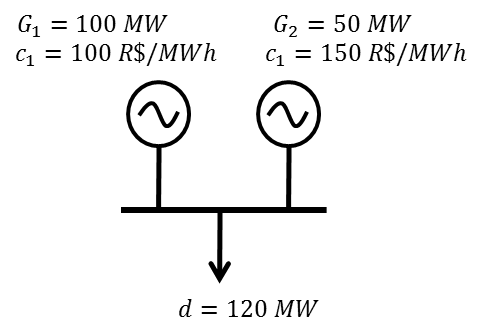
\includegraphics{aula4-1}\protect\caption{\label{fig:aula4-1} Representação gráfica do exemplo }
\end{centering}
\end{figure}
Para atender a demanda com esses dois geradores, uma possível solução para o problema seria utilizar a potência do mais barato e depois, se necessário, utilizar o recurso mais caro. Essa solução é conhecida como ordem de mérito em custo. Será necessário utilizar os $100$MW
do primeiro gerador e completar com $20$MW do segundo gerador para atender a demanda (Figura \ref{fig:aula4-2}).
\begin{figure}[H]
\begin{centering}
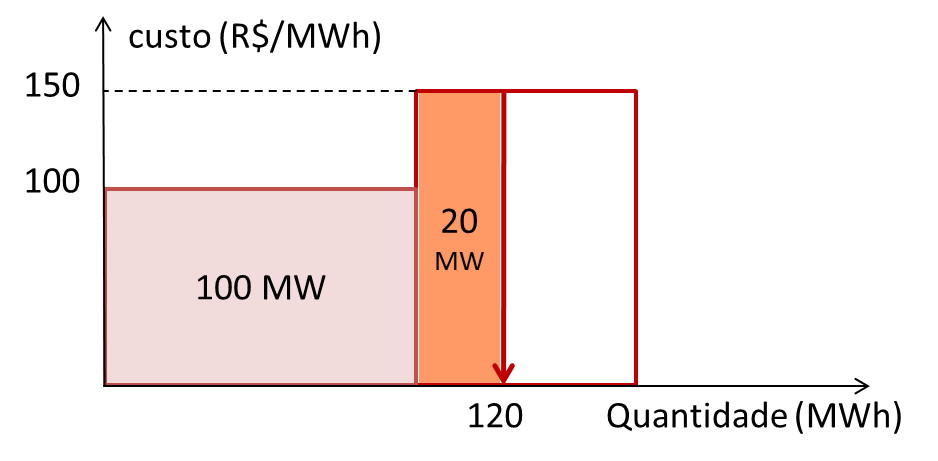
\includegraphics[scale=0.7]{aula4-2}\protect\caption{\label{fig:aula4-2} Despacho por ordem de custo }
\end{centering}
\end{figure}
A modelagem do problema será dado por:
\begin{align}
    & \underset{g\geq0}{\text{Min}} \hspace{1cm} 100g_1+150g_2 \label{eq1} \\
    & \text{s.a}  \hspace{2.2cm} g_1+g_2 \geq 120; \label{eq2} \\
    &             \hspace{2.65cm} g_1\leq 100, \label{eq3}\\
    &             \hspace{2.65cm} g_2\leq 50. \label{eq4}
\end{align}

Na figura \ref{fig:aula4-3}, a área hachurada representa o conjunto de soluções viáveis do problema. Nota-se que em problemas de programação linear (como este em questão) é necessário que o conjunto viável seja um conjunto convexo.
\begin{figure}[H]
\begin{centering}
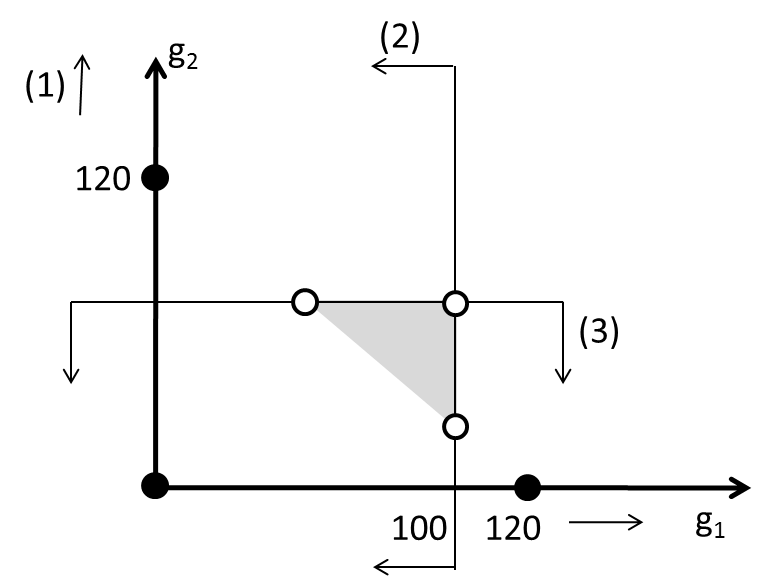
\includegraphics[scale=0.7]{aula4-3}\protect\caption{\label{fig:aula4-3} Gráfico exemplo }
\end{centering}
\end{figure}
\end{exemplo}



Sendo este um problema de minimização, caminhar na direção oposta ao do gradiente fará com que encontremos uma solução melhor do problema. Na figura \ref{fig:aula4-4}, as curvas de nível estão representadas pelas linhas pontilhadas em vermelho, e diminuem no sentido da seta vermelha (direção oposta ao gradiente).

\begin{figure}[H]
\begin{centering}
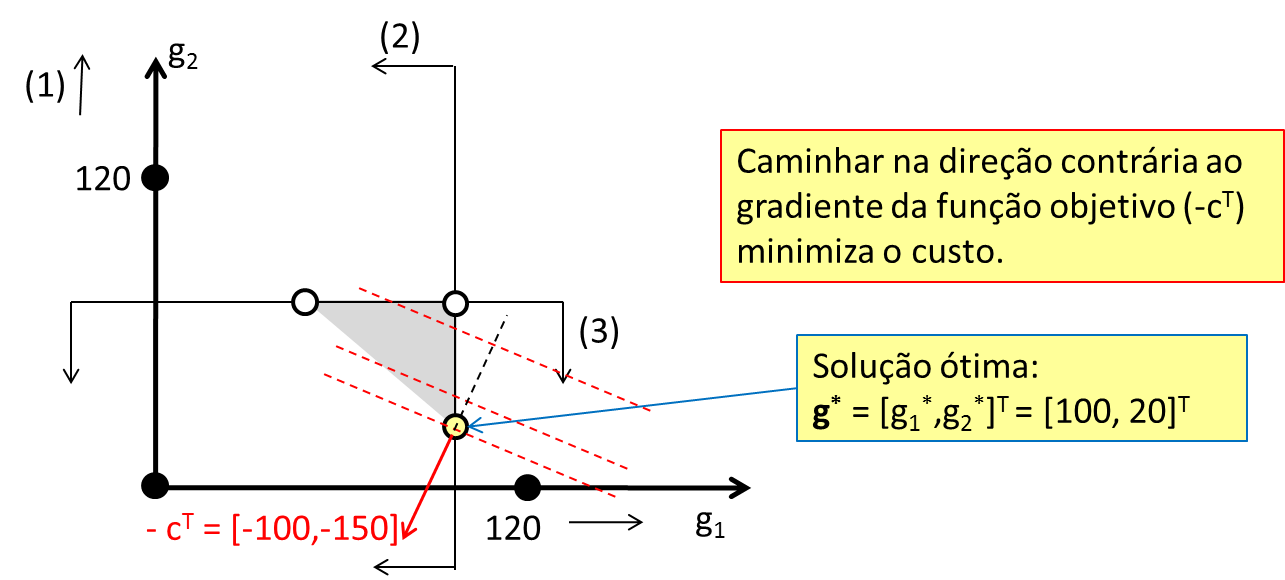
\includegraphics[scale=0.70]{aula4-4}\protect\caption{\label{fig:aula4-4} Gráfico exemplo gradiente }
\end{centering}
\end{figure}

\begin{figure}[H]
\begin{centering}
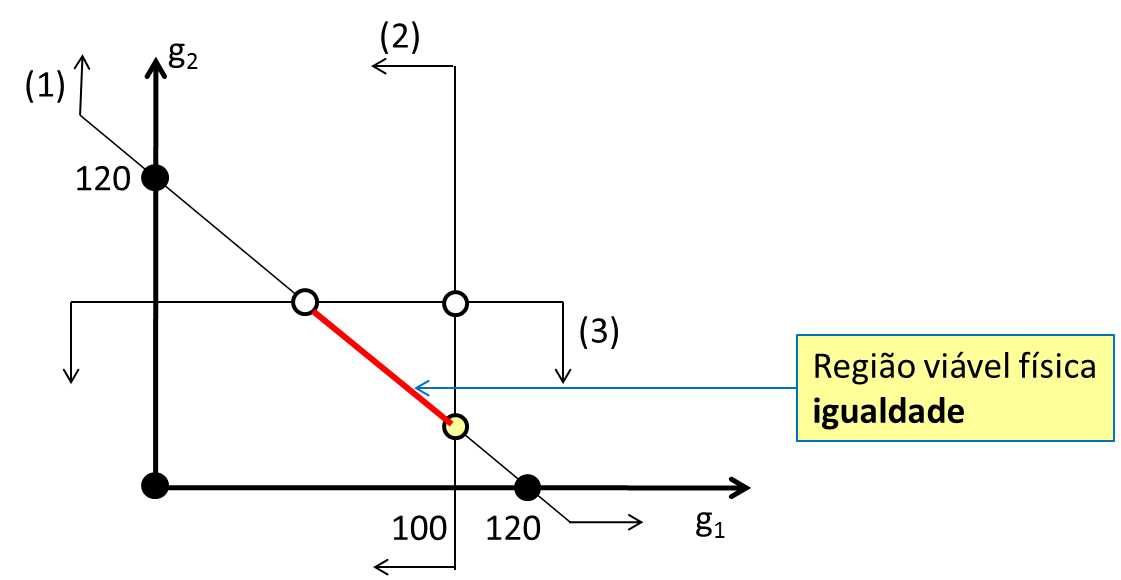
\includegraphics[scale=0.8]{aula4-5}\protect\caption{\label{fig:aula4-5} Gráfico exemplo igualdade}
\end{centering}
\end{figure}

Alterando a restrição de atendimento da demanda (eq. (\ref{eq2})), para uma igualdade, conforme no problema abaixo
\begin{align}
    & \underset{g\geq0}{\text{Min}} \hspace{1cm} 100g_1+150g_2 \label{eq5} \\
    & \text{s.a}  \hspace{2.2cm} g_1+g_2 = 120; \label{eq6} \\
    &             \hspace{2.65cm} g_1\leq 100; \label{eq7}\\
    &             \hspace{2.65cm} g_2\leq 50, \label{eq8}
\end{align}

Através da figura \ref{fig:aula4-5}, é possível concluir que a equação da restrição será alterada, conforme apresentado:\todo{Revisar}
A primeira restrição (\ref{eq6}) é, na verdade, o objetivo primário do nosso problema, já que a mera redução de custo total implicaria em não gerar nada. Assim, a restrição impõe que atendamos a demanda. Claro que, no mundo real, nem sempre é possível atender toda a demanda (picos de demanda ocorrem ou até a falha de algumas geradoras levam aos famosos apagões). Mais adiante, faremos adaptações no modela para levar em consideração esses casos extremos.

O problema de despacho pode ser modelado genericamente da seguinte forma:
\begin{align}
    & \underset{g\geq0}{\text{Min}} \hspace{1cm} \sum_{i=1}^{n}c_{i}\cdot g_{i} \label{eq9} \\
    & \text{s.a}  \hspace{2.2cm} \sum_{i=1}^{n}g_{i}\geq d; \label{eq10} \\
    &             \hspace{2.65cm}g_{i}\leq G_{i}, \quad \forall i=1,...,n. \label{eq11}
\end{align}

Vamos pensar agora em outra análise econômica do problema. Supondo que a demanda precise de um MWh a mais do problema modelado anteriormente, qual o custo deste MWh a ser atendido?
O conceito de usina marginal ou unidade marginal é a usina que está na
margem das usinas que estão produzindo, ou seja, o gerador que irá produzir o próximo MWh no sistema: é aquele que possui o menor custo de produção entre aqueles que ainda possuem capacidade ociosa. 
Este custo marginal pode ser representado por
\[
	\Delta C^{*}(d)=C^{*}(d+1)-C^{*}(d).
\]
Quando a diferença entre a demanda tende a zero, temos a derivada do custo ótimo com relação à demanda:
\[
	\frac{\partial C^{*}(d)}{\partial d}=\lim_{\Delta\rightarrow0^{+}}\frac{C^{*}(d+\Delta-C^{*}(d))}{\Delta} ,
\]
\[
	\frac{\partial C^{*}(d)}{\partial d}=c_{i^{*}},
\]
em que $i^{*}$ é o gerador marginal.
Como no exemplo anterior apenas o gerador 2 possuia potência para atender o
próximo MWh, então o custo para atendê-lo será o custo de geração do gerador 2, isto é, $c_{2}$:
\[
\Delta C^{*}(d)=[C^{*}(d)+c_{2}\cdot1]-C^{*}(d)=c_{2},
\]
Como o problema é resolvido de forma ótima por uma heurística de ordem de mérito, a sua derivada do custo em relação à demanda é uma função escada, com valores iguais aos dos custos de geração em ordem crescente, conforme a figura \ref{fig:aula4-6}.
\begin{figure}[H]
\begin{centering}
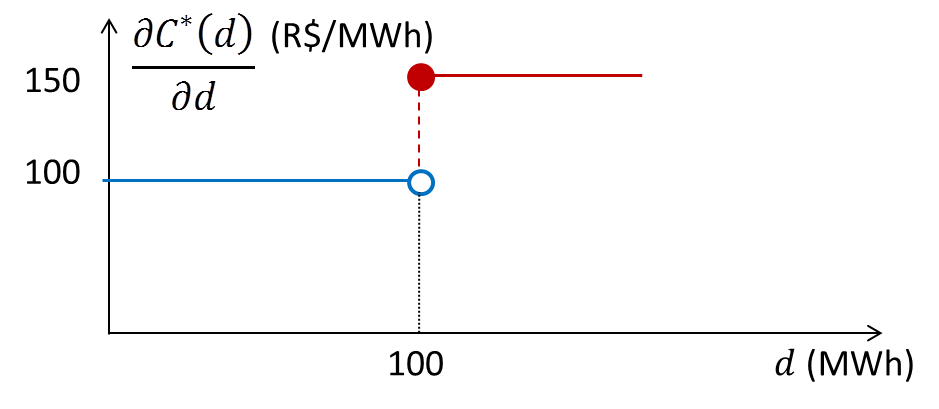
\includegraphics[scale=0.8]{aula4-6}\protect\caption{\label{fig:aula4-6} Derivada nos pontos}
\end{centering}
\end{figure}
Então, aplicado ao exemplo anterior, observamos que o custo do 121º MWh a ser gerado será de R\$150, conforme mostrado na figura \ref{fig:aula4-7}
\begin{figure}[H]
\begin{centering}
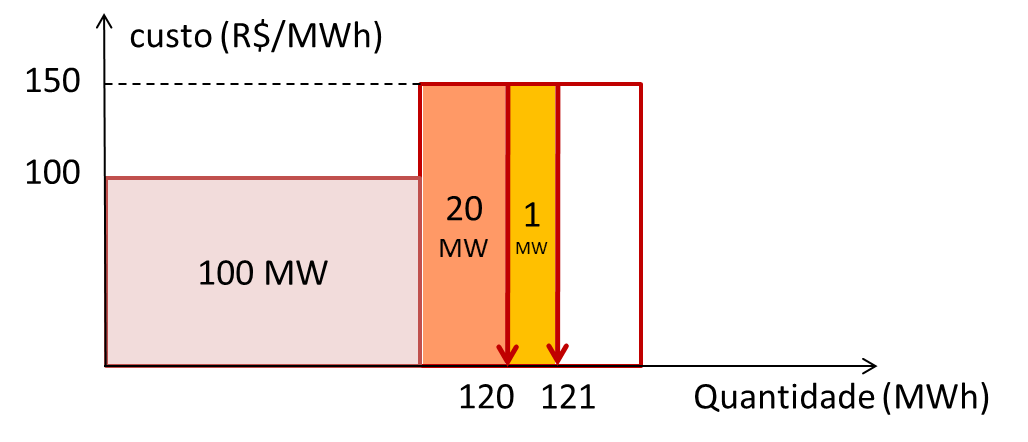
\includegraphics[scale=0.8]{aula4-7}\protect\caption{\label{fig:aula4-7} Gráfico exemplo com custo adicional}
\end{centering}
\end{figure}
A função custo está apresentada na figura (\ref{fig:aula4-8}) e possui as seguintes propriedades importantes:
\begin{itemize}
\item é linear por partes;
\item tem primeira derivada descontínua;
\item é crescente;
\item é convexa.
\end{itemize}
\begin{figure}[H]
\begin{centering}
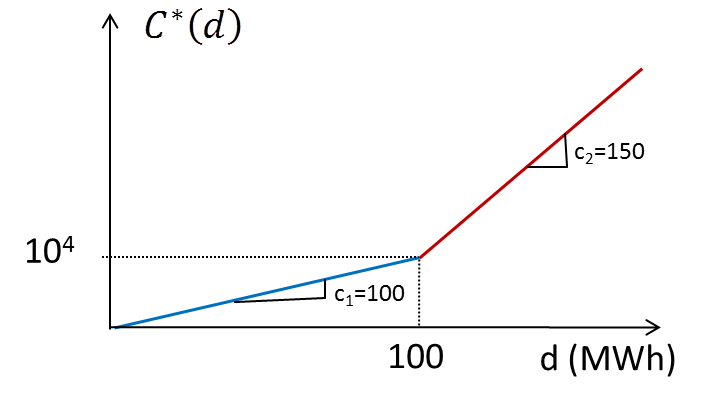
\includegraphics[scale=0.8]{aula4-8}\protect\caption{\label{fig:aula4-8} Função custo}
\end{centering}
\end{figure}



% % % % % % % DUALIDADE % % % %

\subsection{Teoria da dualidade}
%\begin{enumerate}

%%\begin{itemize}
Como funciona o processo de “dualização” de restrições (relaxação langrangeana)?
\begin{equation*}
\begin{aligned}
& z_{p}^{*}=\underset{x\geq0}{\text{Max}}
& & c^{T}x \\
& \text{s.a}
& & Ax \leq b.
\end{aligned}
\end{equation*}
O processo de ``dualização'' implica em relaxar alguma das restrições
(ou todas) do problema primal e incorporar uma penalização na função
objetivo sobre a viabilidade das soluções.
\begin{equation*}
\begin{aligned}
& z_{p}^{*}\leq \theta(y)=\underset{x\geq0}{\text{Max}}
& & c^{T}x+y^{T}(b-Ax)  \\
& \text{s.a}
& & Ax \leq b. \\
& & & \forall  y\geq 0 
\end{aligned}
\end{equation*}
\[
z_{p}^{*}\leq\theta(y)\leq\phi(y)=\max_{x\geq0}c^{T}\cdot x+y^{T}\cdot(b-A\cdot x)\forall y\geq0
\]
\todo[inline]{O que fazer com esses forall y?}
Uma interpretação para a variável dual ($y^{T}(b-A\cdot x)$) é o exemplo dado na aula 1: O dono da fábrica agora pode vender ou comprar a sobra ou déficit de insumos em um mercado (ilimitado) por preço y.
Como se comporta a função dual lagrangeana?

\[
z_{p}^{*}\leq\phi(y)=\max_{x\geq0}c^{T}\cdot x+y^{T}\cdot(b-A\cdot x)\forall y\geq0
\]
 Dado um vetor $y$ de multiplicadores de Lagrange,
\[
z\leq\phi(y)=\max_{x\geq0}(c^{T}-y^{T}\cdot A)\cdot x+y^{T}\cdot b=
\begin{cases}
y^{T}\cdot b, & \mbox{se \ensuremath{c^{T}-y^{T}\cdot A\leq0}}\\
+\infty, & \mbox{c.c.}
\end{cases}
\]
 O processo de relação lagrangeana busca um vetor y que minimize $\phi(y)$. Logo, o segundo caso (que proporciona valor infinito) será sempre evitado. A interpretação para esse comportamento é:
(i) se o lucro unitário de produção $(c^{T})$ for inferior à receita de venda de seus insumos $(y^{T}A)$ no mercado ao preço $y$ , então paramos a produção e vendemos todos os insumos no mercado, resultando em um lucro de $y^{T}b$;
(ii) caso contrário, ocorre a possibilidade de arbitragem, onde podemos comprar no mercado os insumos por preços que geram um custo inferior ao lucro de produção. Nesse caso, compramos infinito e vendemos infinito, obtendo assim uma solução ilimitada.
O problema dual busca um vetor $y$ que minimize $\phi(y)$. Logo, o caso (ii) será sempre evitado.
\[
z\leq\min_{y\geq0}\phi(y)=\min_{y\geq0}
\left\{ \begin{array}{c}
y^{T}\cdot b,sec^{T}-y^{T}\cdot A\leq0\\
+\infty,casocontr\acute{a}rio
\end{array}\right\} =\begin{array}{cc}
\min_{y\geq0} & y^{T}\cdot b\\
s.a: & y^{T}\cdot A\geq c^{T}
\end{array}
\]
Como fazer para descobrir quais são os preços $y$ que minimizam essa função? A busca pelos preços de mercado que deixa o produtor indiferente entre produzir e vender os insumos nos mercados é feita procurando a solução do seguinte problema primal-dual:
\[
z_{p}^{*}=\begin{array}{cc}
\max_{x\geq0} & c^{T}\cdot x\\
s.a: & A\cdot x\leq b
\end{array}\leq z_{d}^{*}=\begin{array}{cc}
\min_{y\geq0} & y^{T}\cdot b\\
s.a: & y^{T}\cdot A\geq c^{T}
\end{array}
\]
 O \textbf{teorema da dualidade fraca} enuncia que (Primal de Maximização):
 \begin{itemize}
 \item O valor mínimo do problema Dual (de minimização) é superior ao máximo do problema primal (de maximização).
 \item Isso torna-se óbvio depois de mostrado o processo de construção do
 dual da maneira que apresentamos aqui. Este foi concebido para sempre
 gerar um limite superior para o problema primal.
 \end{itemize}
Já o \textbf{teorema da dualidade Forte} diz que (Primal de Maximização):
\begin{itemize}
\item No ponto ótimo, o valor da função objetivo de qualquer par primal-dual decorrente de um problema de programação linear é sempre o mesmo, ou seja:
$$
z_{p}^{*}=\begin{array}{cc}
\max_{x\geq0} & c^{T}\cdot x\\
s.a: & A\cdot x\leq b
\end{array} = z_{d}^{*}=\begin{array}{cc}
\min_{y\geq0} & y^{T}\cdot b\\
s.a: & y^{T}\cdot A\geq c^{T}
\end{array}.
$$
\end{itemize}
%\begin{figure}[H]
%\begin{centering}
%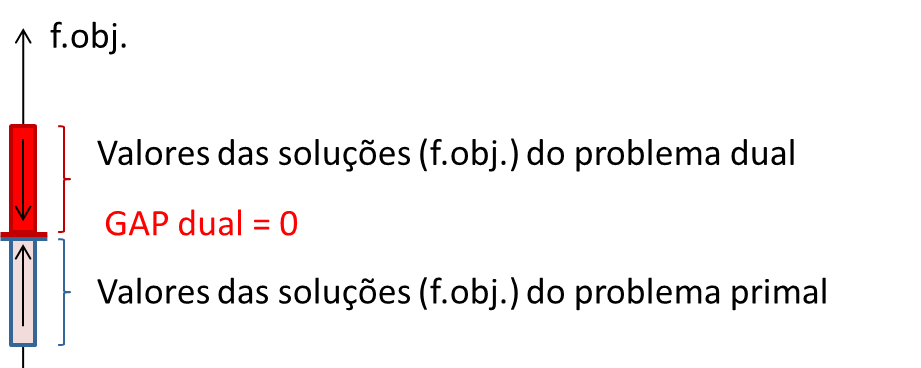
\includegraphics[scale=0.8]{aula4-9}\protect\caption{\label{fig:aula4-9} GAP dual}
%\end{centering}
%\end{figure}
A interpretação mais conhecida e difundida
deste teorema, devido à relação entre o problema primal e o dual,
é a interpretação da variável dual como ``preço sombra'' ou custo
marginal dos recursos. Em problemas convexos, nos quais vale a dualidade forte, a variável dual pode ser interpretada como a derivada parcial do valor ótimo da função objetivo do primal, com relação ao lado direito da restrição associada
a esta variável. Em última análise, é representado pelo multiplicador de Lagrange:
\[
z_{p}^{*}=z_{d}^{*}=y^{*T}\cdot b
\]
\[
\frac{\partial z_{p}^{*}}{\partial b}=\left[\frac{\partial z_{p}^{*}}{\partial b_{1}},...,\frac{\partial z_{p}^{*}}{\partial b_{m}}\right]=\left[y_{1}^{*},...,y_{m}^{*}\right]=y^{*T}.
\]

%\end{itemize}
%\end{enumerate}
\textbf{Exemplo: despacho centralizado vs. competição perfeita}

O despacho ótimo ``centralizado'' de um período, que visa atender uma demanda $d$ (MWh) utilizando os recursos disponíveis (capacidade $G_{i}$) é dado pelo seguinte problema:
\begin{align}
	\underset{g\geq0}{\text{Min}} & \sum_{i=1}^{n}c_{i}\cdot g_{i}\label{eq12}\\
	\text{s.a} & \sum_{i=1}^{n}g_{i}\geq d;\label{eq13}\\
	 & g_{i}\leq G_{i}, \qquad\forall i=1,...,n.\label{eq14}
\end{align}

Para que a solução do problema centralizado corresponda ao custo ótimo na realidade, é importante que os
agentes informem os seus custos operativos e capacidades ($c_{i},G_{i}$) de forma precisa.
Outra alternativa para se determinar as quantidades ótimas de despacho é uma solução na qual se cria um mercado 
da energia. Cada empresa geradora (que é \textit{price-taker}, ou seja, não possui poder de mercado suficiente para influenciar o preço) oferta seus preço (custo real) e quantidade (capacidades máximas), visando maximizar os seus lucros individualmente com a venda de energia através de um leilão de preço uniforme. Observe que a empresa não possui incentivos para mentir seu custo real: se ofertar um preço maior, corre o risco de não conseguir ofertar nada numa situação que poderia ter lucro; e oferecer um preço menor, por motivos óbvios, causaria prejuízo para a empresa. 
Esta solução, que é descentralizada, gera o mesmo custo total que aquele proporcionado pela solução centralizada.

Para montar o problema dual, devemos dualização a restrição de atendimento à demanda em que, para todo $\pi\geq0$, teremos a seguinte relação:
\begin{align*}C^{*}\geq C_{d}^{*}(\pi)= & \underset{g\geq0}{\mbox{Min}}\sum_{i=1}^{n}c_{i}\cdot g_{i}+\pi\cdot\left(d-\sum_{i=1}^{n}g_{i}\right)\\
 & \mbox{s.a. }\,g_{i}\leq G_{i}, \quad \forall i=1,...,n.
\end{align*}

Em seguida, rearranjamos os termos de maneira a colocar as variáveis $g_{i}$ em evidência:
\begin{align*}C^{*}\geq C_{d}^{*}(\pi)= & \underset{g\geq0}{\mbox{Min}}\pi\cdot d-\sum_{i=1}^{n}(\pi-c_{i})\cdot g_{i}\\
 & \mbox{s.a. }\,g_{i}\leq G_{i}, \quad \forall i=1,...,n.
\end{align*}

Como o primeiro termo não depende da decisão $g$, este pode ser colocado fora da  minimização e podemos verificar que o $\min$ de uma função negativa é o $\max$ desta função colocando o sinal de negativo para fora da função $\max$. Temos que:

\begin{align*}C^{*}\geq C_{d}^{*}(\pi)= & \pi\cdot d-\sum_{i=1}^{n}Max_{g\geq0_{i}}(\pi-c_{i})\cdot g_{i}\\
 & \mbox{s.a. }\,g_{i}\leq G_{i}, \quad \forall i=1,...,n.
\end{align*}
Por fim, repare que o problema de minimização pode ser decomposto
em $n$ problemas, em que cada um pode ser substituído por um de maximização.

Assim, dado o preço do mercado $\pi$ é encontrado o problema de maximização da receita líquida de venda ($\max_{g\geq0_{i}}(\pi-c_{i})\cdot g_{i}$).
O problema resultante é o problema em que cada agente gerador visa maximizar a sua renda vendendo energia a um preço $\pi$(R\$/MWh) e a demanda (inelástica) paga o mesmo preço pela aquisição dessa energia.
Temos, então, o modelo abaixo:
\[
C^{*}\geq Max_{\pi\geq0}\pi\cdot d-\sum_{i=1}^{n}R_{i}^{*}(\pi)
\]

\begin{align*}R_{i}^{*}(\pi)= & Max_{g_{i}\geq0}(\pi-c_{i})\cdot g_{i}\\
 & \mbox{s.a. }\,g_{i}\leq G_{i},\quad\forall i=1,...,n.
\end{align*}
 

\begin{figure}[H]
\begin{centering}
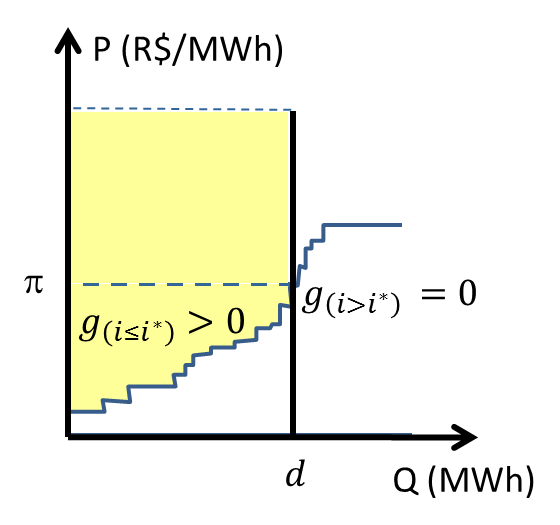
\includegraphics[scale=0.8]{aula4-10}\protect\caption{\label{fig:aula4-10} Operação centralizada vs competitiva}
\end{centering}
\end{figure}
Se a demanda for maior que a soma das capacidades máximas disponíveis no momento, então o
problema é inviável. Graficamente, a situação é apresentada na figura \ref{fig:aula4-10}. 
\begin{figure}[H]
\begin{centering}
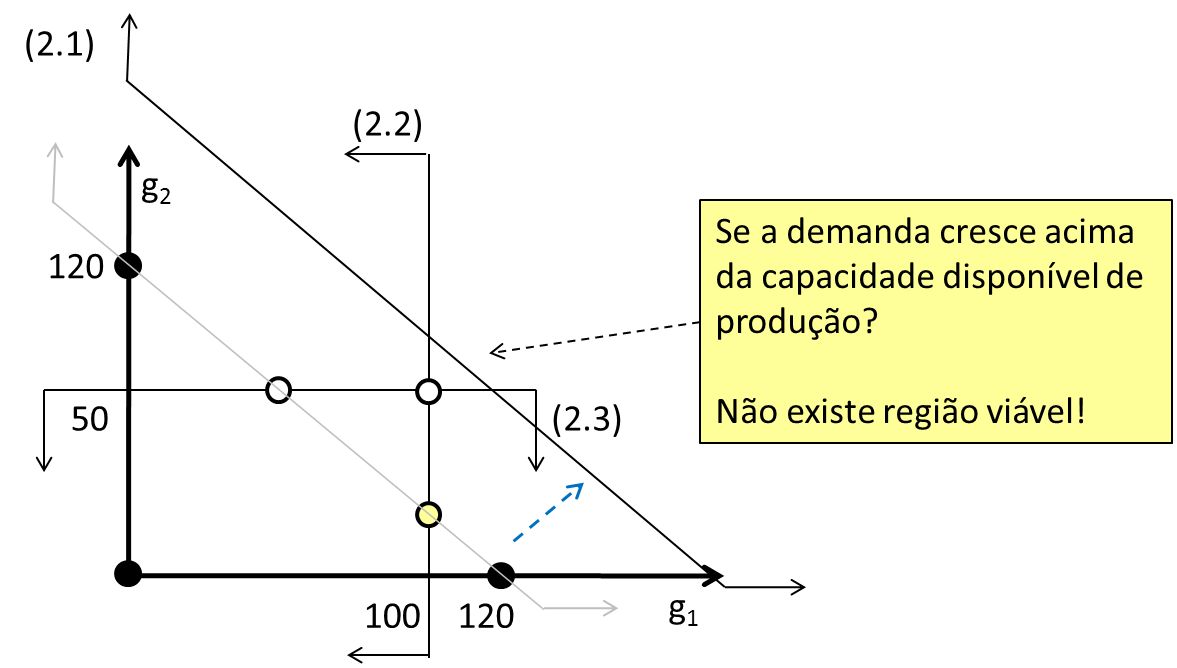
\includegraphics[scale=0.5]{aula4-11}\protect\caption{\label{fig:aula4-11} Gráfico com o aumento da demanda}
\end{centering}
\end{figure}
É preciso, portanto, modificar o problema de forma que ele possa ser otimizado, e não retorne apenas um aviso de que ele é inviável, já que na prática devemos ter uma geração e suprir parte da demanda. Devemos realizar, portanto, um ``corte de carga'' ou déficit (diferente de racionamento). Na realidade, o sistema é operado cortando algumas cargas (diminuindo as cargas), como por exemplo de uma área da distribuidora, desligando alguns consumidores. Graficamente, devemos ter uma adaptação como mostrado na figura \ref{fig:aula4-12}.
\begin{figure}[H]
\begin{centering}
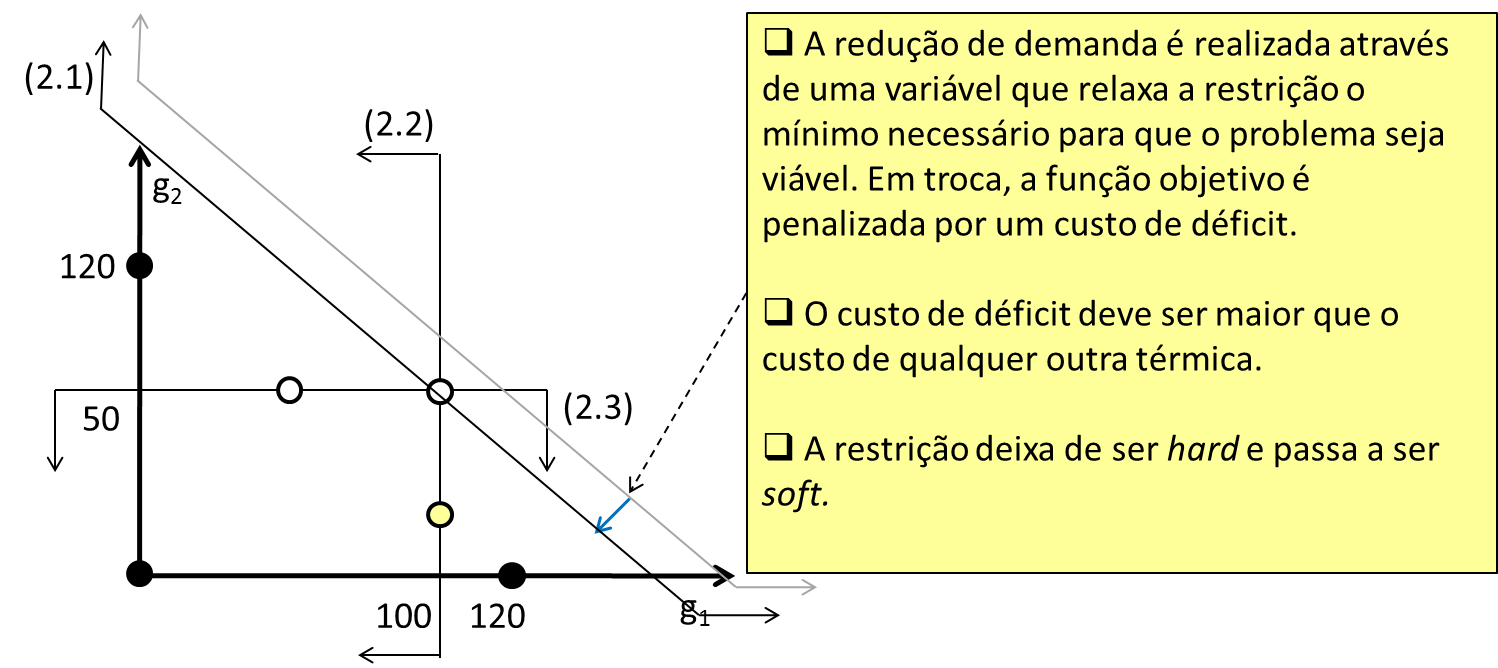
\includegraphics[scale=0.7]{aula4-12}\protect\caption{\label{fig:aula4-12} Viabilidade do problema}
\end{centering}
\end{figure}
Caso falte capacidade de produção, será necessário transformar um restrição hard (inicialmente a restrição de atender à demanda) para um restrição suavizada (atender a demanda sempre que possível) então será necessário diminuir a demanda assim, esse corte de carga é ótimo. 
Para isso introduzimos uma variável ao problema que age como se
fosse um gerador, porem é um corte de carga.Essa variável adicionada ao problema  é uma variável de decisão e é penalizada no problema na função objetivo com um custo de deficit maior que o custo dos outros geradores.
Assim é possível construir a curva de déficit, com diferente patamares
que será modelado na seguinte maneira:
\begin{align}
    & \underset{g\geq0, r\geq0}{\text{Min}} \hspace{1cm} \sum_{i=1}^{n}c_{i}\cdot g_{i} + c_{d}\cdot r \label{eq15} \\
    & \text{s.a}  \hspace{2.2cm} \sum_{i=1}^{n}g_{i} + r\geq d \label{eq16} \\
    &             \hspace{2.65cm}g_{i}\leq G_{i}, \quad \forall i=1,...,n,\label{eq17}
\end{align}
mm que $c_d$ é o custo do déficit por unidade e $r$ o tamanho do déficit.
Se o desejo é modelar uma função convexa para o custo do déficit, podemos escrevê-la como uma função linear por partes, e o custo $c_d$ se transforma num vetor de custos $\{c_j^d\}$ para os diferentes componentes (ver a figura \ref{fig:aula4-14}).
Essa função é conhecida como custo de déficit e o modelo que o implementa é apresentado a seguir:
\begin{align}
    & \underset{g\geq0, r\geq0}{\text{Min}} \hspace{1cm} \sum_{i=1}^{n}c_{i}\cdot g_{i} + \sum_{j=1}^{m}c_{j}^{d}\cdot r_{j} \label{eq16} \\
    & \text{s.a}  \hspace{2.2cm} \sum_{i=1}^{n}g_{i} + \sum_{j=1}^{m}r_{j}\geq d \label{eq17} \\
    &             \hspace{2.65cm}g_{i}\leq G_{i} \forall i=1,...,n\label{eq18}\\
    &                \hspace{2.65cm}r_{j}\leq \bar{r}_{j} \forall j=1,...,m.\label{eq19}
\end{align}
\begin{figure}[H]
\begin{centering}
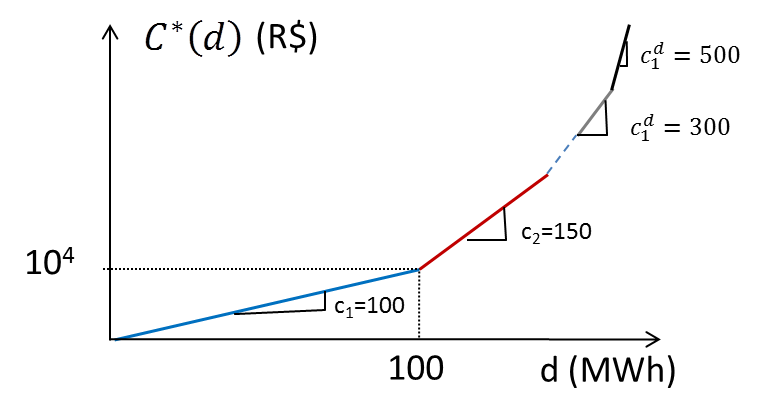
\includegraphics[scale=0.8]{aula4-14}\protect\caption{\label{fig:aula4-14} Função custo com o custo de déficit }
\end{centering}
\end{figure}
\todo[inline]{Reescrever parágrafo}
A figura (\ref{fig:aula4-15}) é conhecida como curva de duração de demanda. No eixo $x$ está representada a frequência no ano e on eixo $y$ está representada a demanda. Uma interpretação para este gráfico é que quando a demanda atingir uma carga crítica de, por exemplo, ($5\%$) em uma duração de ($5\%$) do ano, estaríamos utilizando geradores flexíveis, geradores de base e geradores inflexível. 
Geradores de bases praticamente inflexível (exemplo:nuclear e carvão) produzem energia ($100\%$) durante o ano e possuem custo de investimento caro e custo de operação barato ou seja, são os primeiro a serem ligados. Geradores de bases flexíveis conseguem gerar e desligar se necessário com um taxa de desligamento (não acionamento), às vezes a demanda fica menor do que o custo variável destes. Geradores flexíveis  são responsáveis por atender demandas no intervalo acima, o os demais geradores são conhecidos como geradores de pico que vivem para atender aproximadamente 3\% da carga. Só em eventos raros ele será acionado para produzir. Porem,qual deve ser o valor que se paga para os geradores de pico para produzir sabendo que eles vão produzir em poucas horas.
\begin{figure}[H]
\begin{centering}
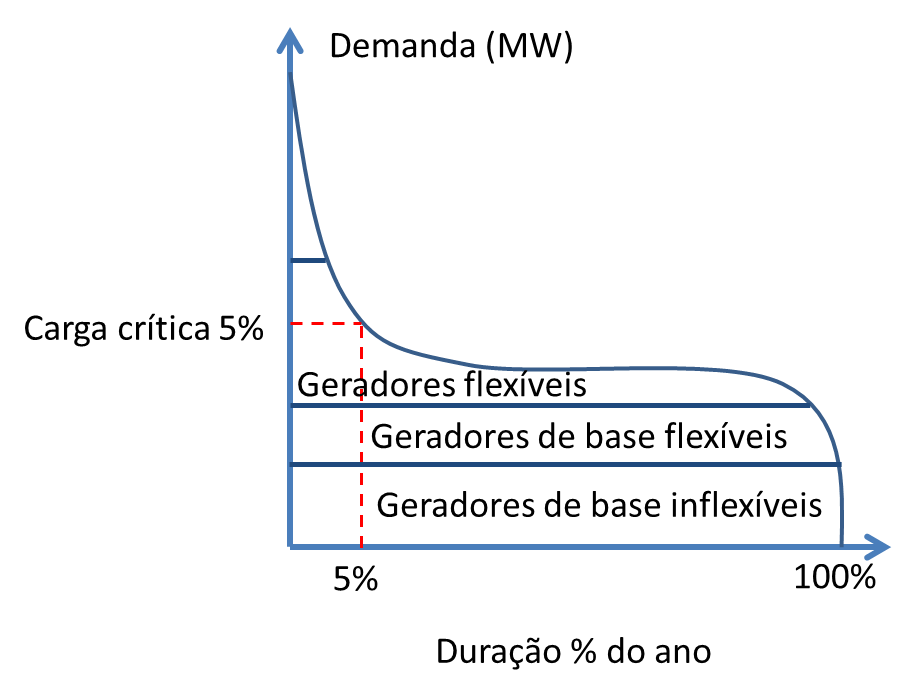
\includegraphics[scale=0.7]{aula4-15}\protect\caption{\label{fig:aula4-15}  Curva de duração de demanda}
\end{centering}
\end{figure}

\subsection{Restrições de rede}
\textbf{Exemplo}

Sejam dois geradores em locais diferentes ligados por uma linhas de transmissão em que os geradores possuam capacidades finitas e limites de transmissão. O gerador $1$ tem capacidade máxima de produção de $100$ MW e o custo de $100$R\$/MWh, enquanto o  gerador $2$  tem capacidade máxima de produção de $50$ MW e o custo de $150$R\$/MWh. Esses geradores precisam atender uma demanda de $120$MW (esquema na figura \ref{fig:aula4-16}). O diferencial deste exemplo para o exemplo apresentando anteriormente está na linha de transmissão. O gerador $1$ pode transmitir $80$ MW e a linha de transmissão do gerador $2$ pode passar $80$MW para atender a demanda de $120$MW.
\begin{figure}[H]
\begin{centering}
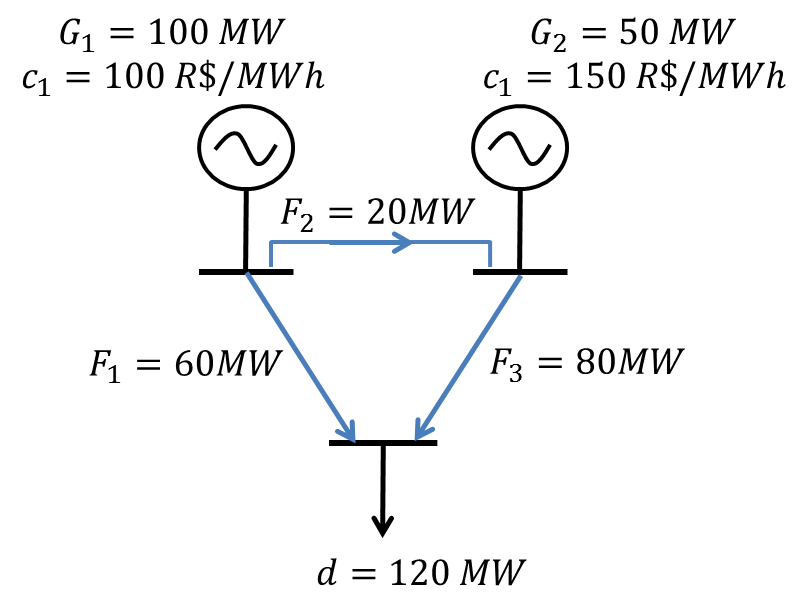
\includegraphics[scale=0.8]{aula4-16}\protect\caption{\label{fig:aula4-16} Exemplo ligado por linha de transmissão}
\end{centering}
\end{figure}
O despacho ótimo encontrado no primeiro exemplo, de $g_{1}^{*}=100$, não pode ser injetado na rede; neste caso, portanto, a solução será inviável.
A seta na (Figura \ref{fig:aula4-16}) representa o sentido do fluxo. Por convenção adotaremos que quando a senta sai do gerador perde energia.

O \textbf{modelo de transporte}, possui esse nome por não considerar algumas características elétricas da rede. A restrição de atendimento à demanda (balanço de potência ou nodal) por barra para o exemplo apresentado é dada pelas equações:
\[
	g_{1}-f_{1}-f_{2}=0,
\]
\[
	g_{2}+f_{2}-f_{3}=0,
\]
\[
	f_{1}+f_{3}=d.
\]
O sinal do fluxo depende da convenção: (+) se passa no sentido das setas e (-) caso contrário.
Então, a restrição de capacidade das linhas é dada pela restrição:
\[
-F_{l}\leq f_{1}\leq F_{l}.
\]
Quando reorganizamos as restrições para visualização em formato de matriz, temos a matriz de incidência de fluxo em redes, em que definimos $+1$ como o coeficiente se a aresta $l$ chega
no vértice $i$ e $-1$ se sai:
\[
\begin{array}{ccccccc}
g_{1} &  & -f_{1} & -f_{2} &  & = & 0,\\
 & g_{2} &  & +f_{2} & -f_{3} & = & 0,\\
 &  & f_{1} &  & +f_{3} & = & d.
\end{array}
\]
Ou seja, tudo que entra na barra é igual a tudo que sai dessa barra.
Assim, podemos montar o modelo de transporte completo do exemplo:
\[
	\min_{g_{i}\geq0,f_{l}}100g_{1}+150g_{2}
\]
\[
\begin{array}{ccccccc}
s.a:\\
g_{1} &  & -f_{1} & -f_{2} &  & = & 0\\
 & g_{2} &  & +f_{2} & -f_{3} & = & 0\\
 &  & f_{1} &  & +f_{3} & = & d\\
-60 & \leq & f_{1} &  &  & \leq & 60\\
-20 & \leq &  & f_{2} &  & \leq & 20\\
-80 & \leq &  &  & f_{3} & \leq & 80\\
g_{1} &  &  &  &  & \leq & 100\\
 & g_{2} &  &  &  & \leq & 50.
\end{array}
\]
A Figura (\ref{fig:aula4-17}) apresenta a solução ótima do problema.
\begin{figure}[H]
\begin{centering}
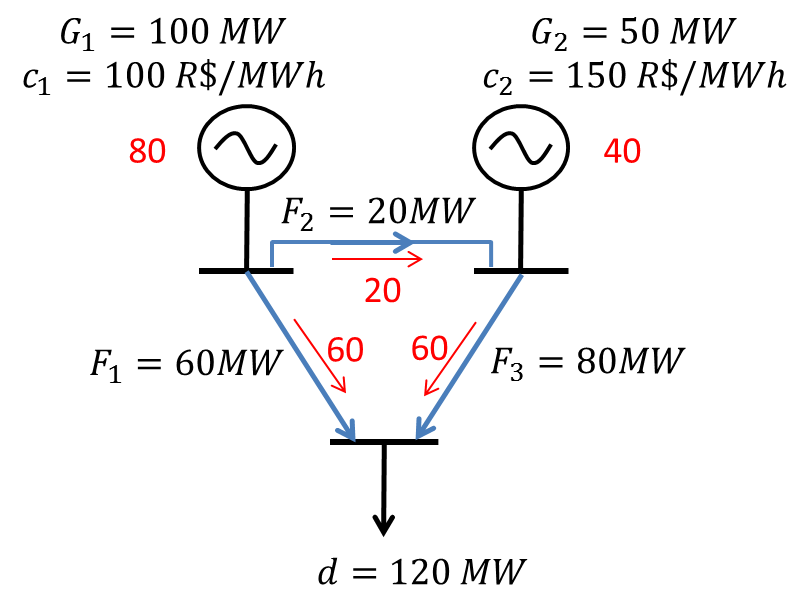
\includegraphics[scale=0.7]{aula4-17}\protect\caption{\label{fig:aula4-17} Solução ótima do exemplo}
\end{centering}
\end{figure}


Conhecemos por \textbf{custo marginal nodal} o custo de atender $1$ MWh a mais, sendo que neste exemplo podemos adicionar esse MWh para cada barra do sistema.
No caso da barra $1$, o custo adicional de operação ótima para suprir $1$ MWh está representado na figura (\ref{fig:aula4-18}) e  modelado da seguinte maneira:
\[
\min_{g_{i}\geq0,f_{l}}100g_{1}+150g_{2}
\]
\[
\begin{array}{ccccccc}
s.a:\\
g_{1} &  & -f_{1} & -f_{2} &  & = & +1\\
 & g_{2} &  & +f_{2} & -f_{3} & = & 0\\
 &  & f_{1} &  & +f_{3} & = & d\\
-60 & \leq & f_{1} &  &  & \leq & 60\\
-20 & \leq &  & f_{2} &  & \leq & 20\\
-80 & \leq &  &  & f_{3} & \leq & 80\\
g_{1} &  &  &  &  & \leq & 100\\
 & g_{2} &  &  &  & \leq & 50.
\end{array}
\]

\begin{figure}[H]
\begin{centering}
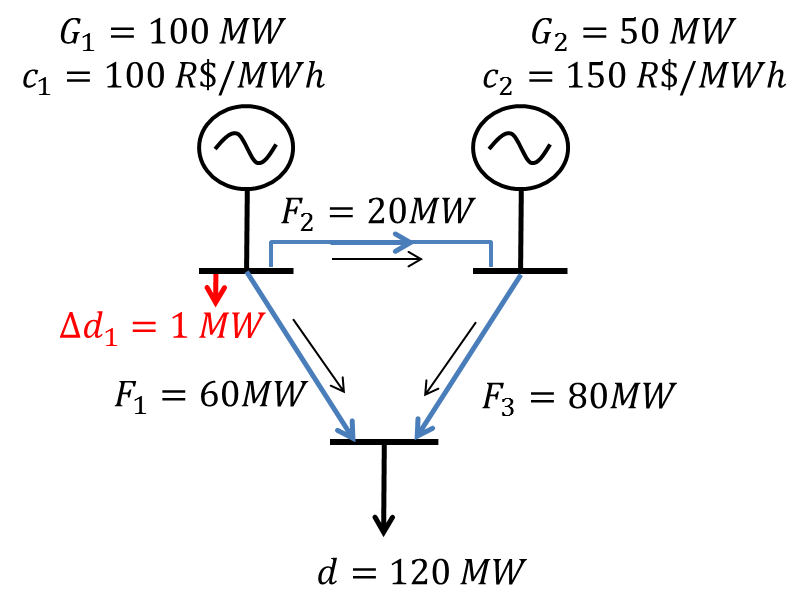
\includegraphics[scale=0.7]{aula4-18}\protect\caption{\label{fig:aula4-18} Aumento da demanda na barra 1}
\end{centering}
\end{figure}
O custo adicional de operação encontrada é de $\pi_{1}=100$ R$\$$/MWh representado na figura (\ref{fig:aula4-19} ).
\begin{figure}[H]
\begin{centering}
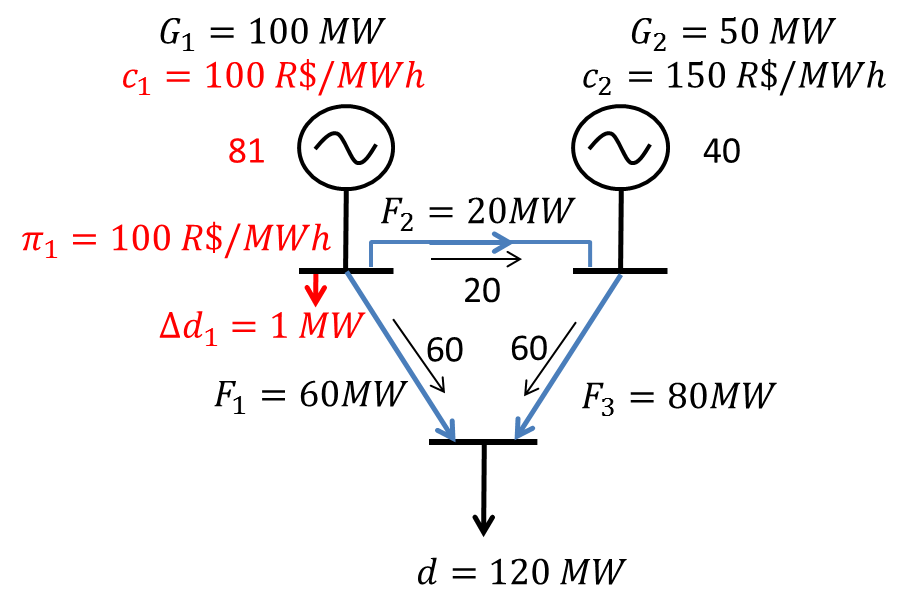
\includegraphics[scale=0.7]{aula4-19}\protect\caption{\label{fig:aula4-19} Custo adicional na barra 1 }
\end{centering}
\end{figure}
Na barra $2$, o custo adicional de operação ótima para suprir $1$ MWh está representado na figura (\ref{fig:aula4-20}) e a modelagem dada por:
\[
\min_{g_{i}\geq0,f_{l}}100g_{1}+150g_{2}
\]
\[
\begin{array}{ccccccc}
s.a:\\
g_{1} &  & -f_{1} & -f_{2} &  & = & 0\\
 & g_{2} &  & +f_{2} & -f_{3} & = & +1\\
 &  & f_{1} &  & +f_{3} & = & d\\
-60 & \leq & f_{1} &  &  & \leq & 60\\
-20 & \leq &  & f_{2} &  & \leq & 20\\
-80 & \leq &  &  & f_{3} & \leq & 80\\
g_{1} &  &  &  &  & \leq & 100\\
 & g_{2} &  &  &  & \leq & 50.
\end{array}
\]

\begin{figure}[H]
\begin{centering}
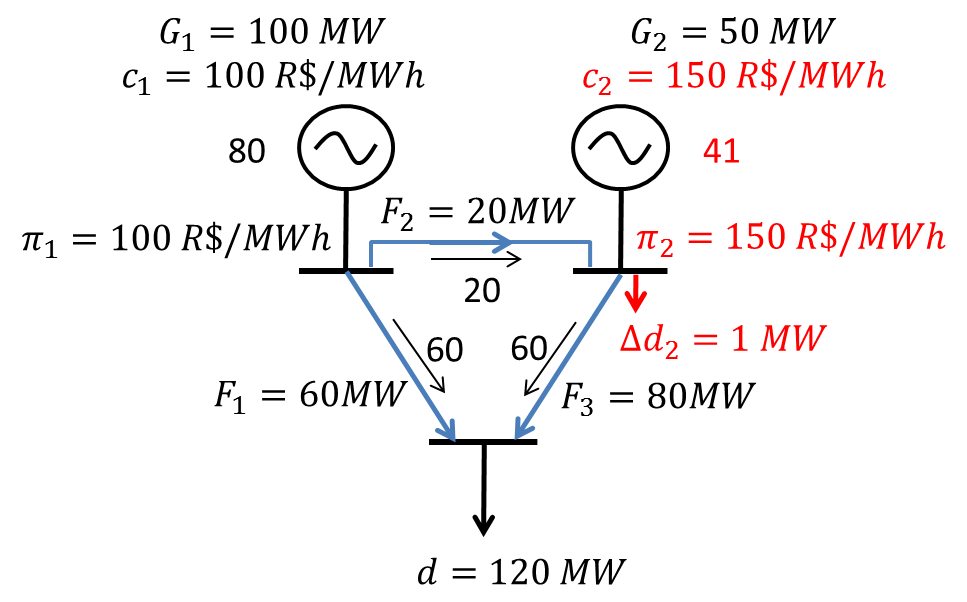
\includegraphics[scale=0.7]{aula4-20}\protect\caption{\label{fig:aula4-20} Custo adicional na barra 2}
\end{centering}
\end{figure}

Então, o custo adicional de operação encontrada é de  $\pi_{2}=150$ R$\$$/MWh.
Ao adicionar $1$ MWh na demanda, a barra $2$ irá atender essa demanda extra sem necessidade de cortar carga, conforme apresentado na figura (\ref{fig:aula4-21}).
\[
\min_{g_{i}\geq0,f_{l}}100g_{1}+150g_{2}
\]
\[
\begin{array}{ccccccc}
s.a:\\
g_{1} &  & -f_{1} & -f_{2} &  & = & 0\\
 & g_{2} &  & +f_{2} & -f_{3} & = & 0\\
 &  & f_{1} &  & +f_{3} & = & d+1\\
-60 & \leq & f_{1} &  &  & \leq & 60\\
-20 & \leq &  & f_{2} &  & \leq & 20\\
-80 & \leq &  &  & f_{3} & \leq & 80\\
g_{1} &  &  &  &  & \leq & 100\\
 & g_{2} &  &  &  & \leq & 50.
\end{array}
\]

\begin{figure}[H]
\begin{centering}
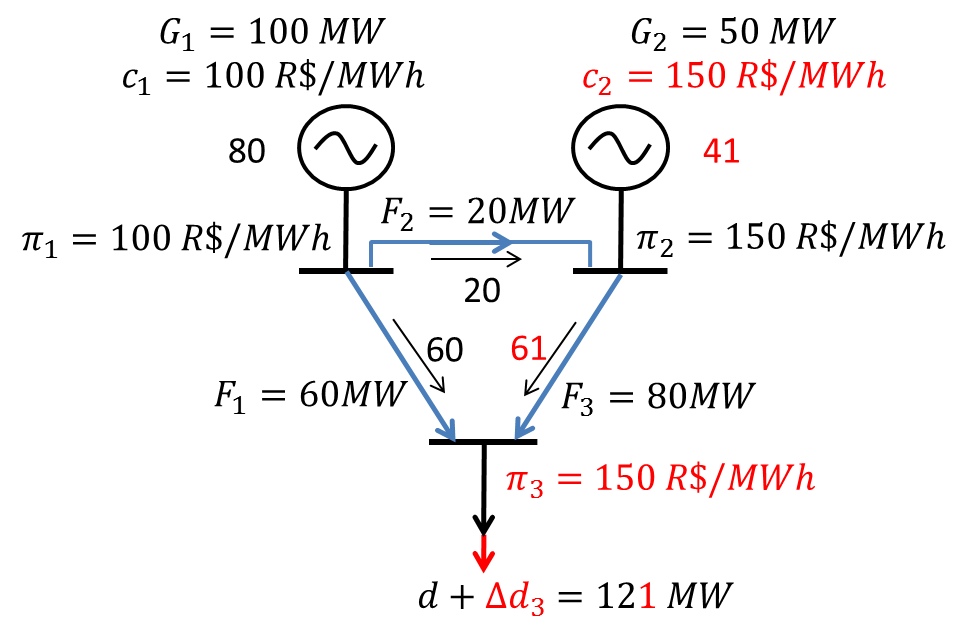
\includegraphics[scale=0.8]{aula4-21}\protect\caption{\label{fig:aula4-21} Custo adicional na demanda}
\end{centering}
\end{figure}

De maneira geral podemos associar os  $\pi_{i}$ (variáveis duais destas restrições do ponto ótimo do dual), da seguinte forma:
\[
\min_{g_{i}\geq0,f_{l}}100g_{1}+150g_{2}
\]
\[
\begin{array}{ccccccc}
s.a:\\
g_{1} &  & -f_{1} & -f_{2} &  & = & 0 (\pi_{1}) \\
 & g_{2} &  & +f_{2} & -f_{3} & = & 0 (\pi_{2})\\
 &  & f_{1} &  & +f_{3} & = & d (\pi_{3})\\
-60 & \leq & f_{1} &  &  & \leq & 60\\
-20 & \leq &  & f_{2} &  & \leq & 20\\
-80 & \leq &  &  & f_{3} & \leq & 80\\
g_{1} &  &  &  &  & \leq & 100\\
 & g_{2} &  &  &  & \leq & 50.
\end{array}
\]

No \textbf{modelo DC linearizado}, adicionamos mais uma restrição ao problema,sendo esta uma restrição linearizada do fluxo de potência visto na aula 3.
Para isso, devemos incorporar a segunda lei de Kirchhoff:
\[
	f_{l}=\frac{1}{x_{l}}(\theta_{ori(l)}-\theta_{des(l)}),
\]
o fluxo numa linha ($f_{l}$) é proporcional ao inverso da reatância ($x_{l}$) e à diferença de ângulos entra as barras ($\theta_{ori(l)}-\theta_{des(l)}$). 
Supondo $x_{l}=1$:
$$f_{1}=\theta_{1}-\theta_{3},$$
$$f_{2}=\theta_{1}-\theta_{2},$$
$$f_{3}=\theta_{2}-\theta_{3}.$$
Assim, temos uma restrição por ciclo:
$$f_{1}=\theta_{1}-\theta_{3},$$
$$f_{2}=\theta_{1}-\theta_{2},$$
$$f_{3}=\theta_{2}-\theta_{3}.$$

Criando, então, uma dependência linear dos fluxos. Logo, $f_{2}=f_{1}-f_{3}$.
Devido a restrição acima e ao limite do fluxo na linha 2, temos: $-20\leq f_{1}-f_{3} \leq 20$.

O despacho ótimo sem rede é inviável mesmo que exista capacidade suficiente
de transmissão.
Agora, supondo que ampliemos a capacidade de $f_{1}$. Pela dependência, este problema não
é viável, dado que $100-20=80$, o que não atende a restrição de $-20\leq f_{1}-f_{3}\leq20$ (Figura \ref{fig:aula4-22}).

\begin{figure}[H]
\begin{centering}
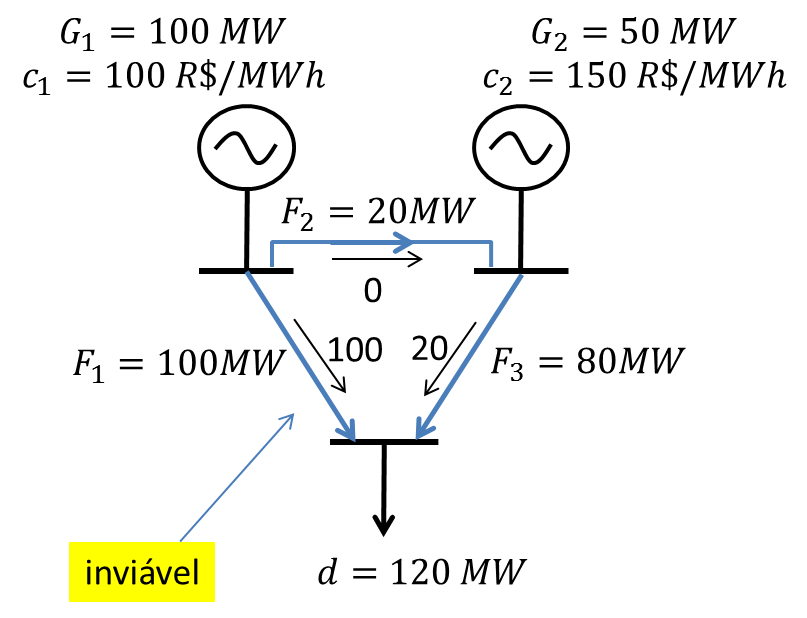
\includegraphics[scale=0.6]{aula4-22}\protect\caption{\label{fig:aula4-22} Problema inviável}
\end{centering}
\end{figure}

\subsection{Confiabilidade}
%%\begin{itemize}
 Frequentes apagões demonstram que a confiabilidade do sistema ainda é um tema não resolvido. Os níveis de reserva (baixos) colocam o sistema em risco mesmo sob contingências corriqueiras.  Falhas em cascata são uma das principais causas de grandes apagões. Além disso, as redes elétricas são frequentes alvos de ataques ou de roubo.

\begin{figure}[h]
\begin{centering}
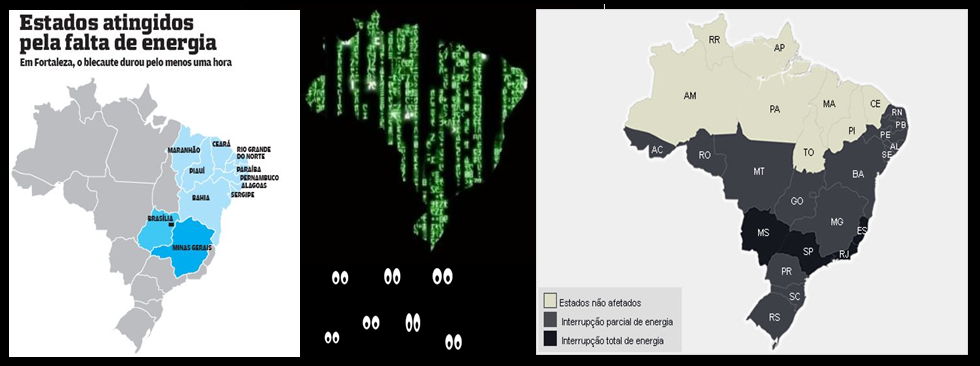
\includegraphics[scale=0.8]{aula4-23}\protect\caption{\label{fig:aula4-23} Apagões}
\end{centering}
\end{figure}
\begin{figure}[h]
\begin{centering}
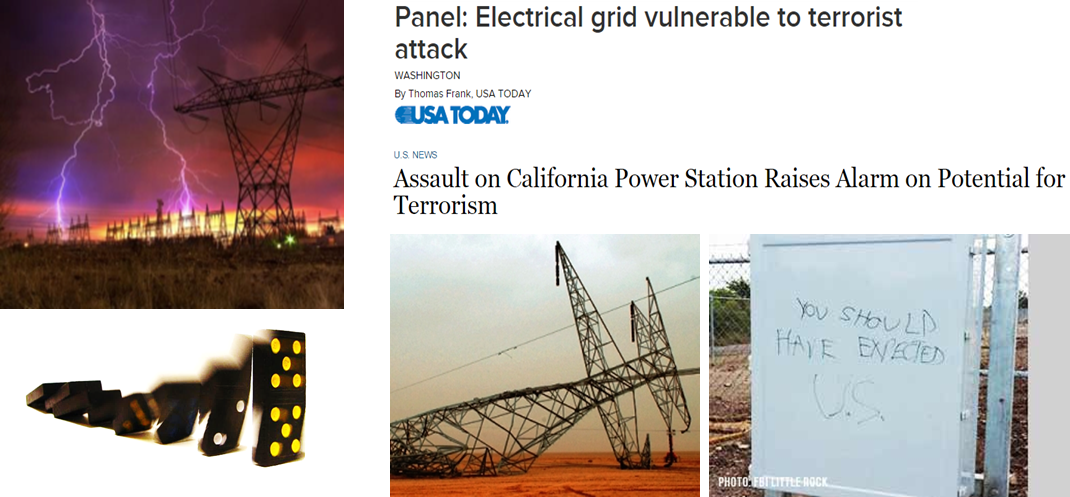
\includegraphics[scale=0.8]{aula4-24}\protect\caption{\label{fig:aula4-24} Falhas em cascata e ataques a redes elétricas }
\end{centering}
\end{figure}
%\end{itemize}

Então, é necessário garantir o suprimento da demanda com algum critério de "confiança". Uma possibilidade para isso é associar uma probabilidade para os eventos de falha: $Prob(\text{Demanda não suprida} > 0)\leq3\%$.
Ou seja, o corte de carga deve ser positivo e limitado.
Se a probabilidade de um dos geradores falhar é $5\%$ e as falhas
são independentes:

$$P(\text{Falhar G1 e G2})=1-((1-P(\text{Falhar G1}))\cdot (1-P(\text{Falhar G2})))= 1-((1- 0.05) \cdot (1-0.05)) = 1- 0.95^2 = 9.75\%,$$
Dado que os dois geradores são necessários para suprir a demanda. Logo, devemos garantir que o sistema tenha reserva suficiente para suprir a demanda mesmo que um gerador falhe. Este é o critério $n-1$ de segurança. 

Serviços ancillares são as principais reservas girantes (capacidade ociosa nos geradores acoplados que permitem o sistema retomar o equilíbrio, frequência e tensão, através do ``redespacho'' dos geradores remanescentes).
O modelo de despacho econômico de potência e reservas (Figura \ref{fig:aula4-25}) tem como objetivo alocar as reservas de maneira que elas sejam entregáveis e garantem a entregabilidade das reservas mesmo que um gerador falhe. 
\textbf{Programação pré-contingência} (ou programação nominal) é a programação caso nada de inesperado aconteça. Para garantir a confiabilidade, devemos deixar uma quantidade de energia em reserva para ser utilizada pelos geradores caso algo falhe. Essa quantidade de reserva é expressa no modelo como as variáveis $r_i$,  sendo que o custo da reserva é não-nulo.

\begin{figure}[H]
\begin{centering}
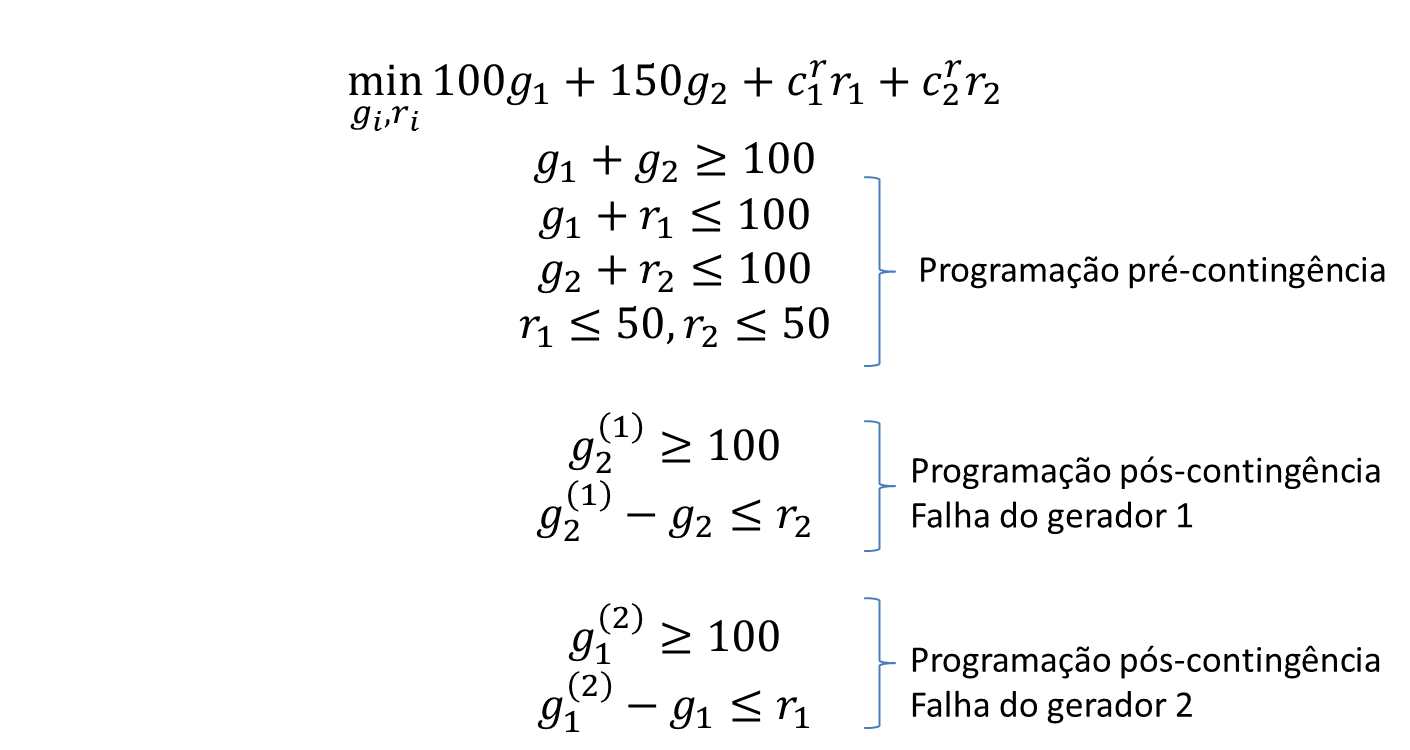
\includegraphics[scale=0.5]{aula4-25}\protect\caption{\label{fig:aula4-25} Modelo de despacho econômico de potência e reservas }
\end{centering}
\end{figure}


\begin{figure}[H]
\begin{centering}
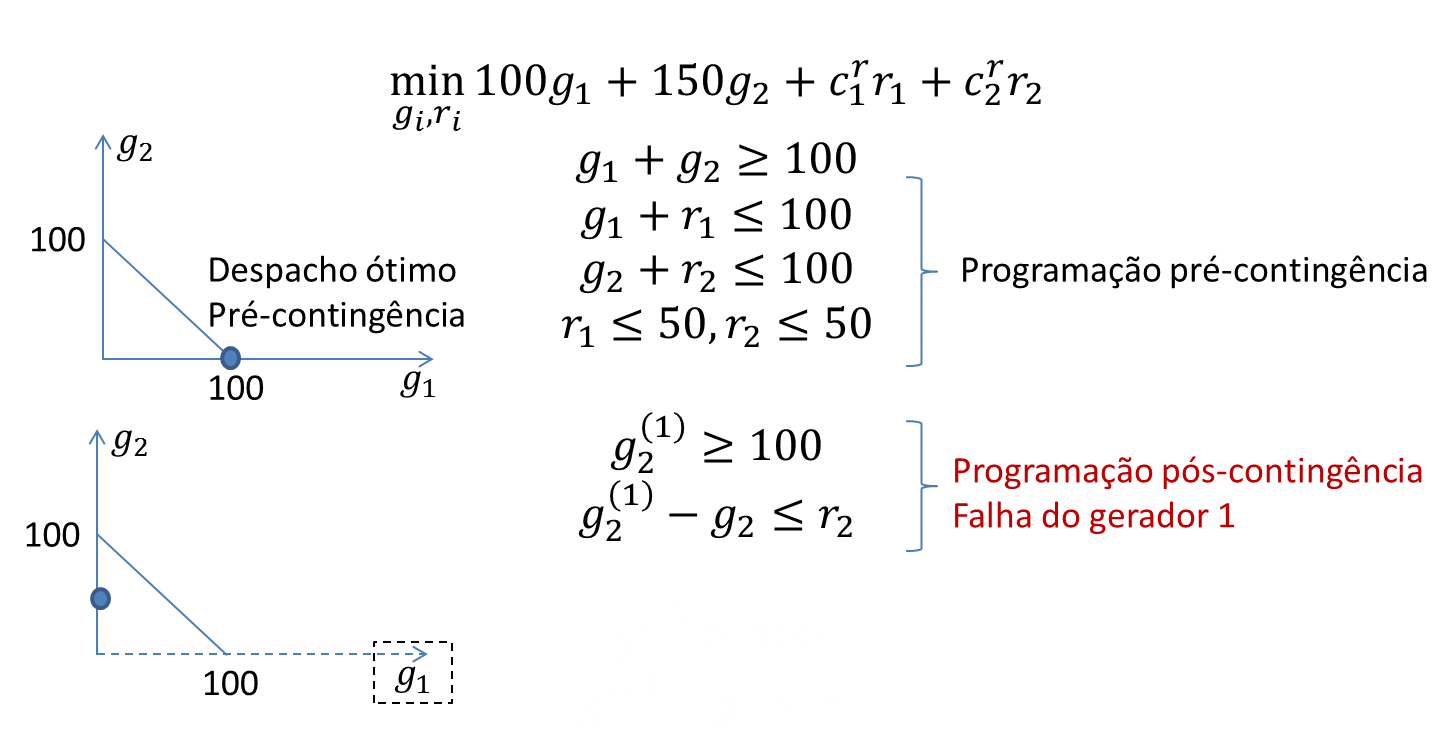
\includegraphics[scale=0.5]{aula4-26}\protect\caption{\label{fig:aula4-26} Falha do gerador 1}
\end{centering}
\end{figure}
Na figura \ref{fig:aula4-27}, o redespacho viável dentro das reservas programadas para atender a carga de $100$ Mw em qualquer estado pós-contingência. 

\begin{figure}[H]
\begin{centering}
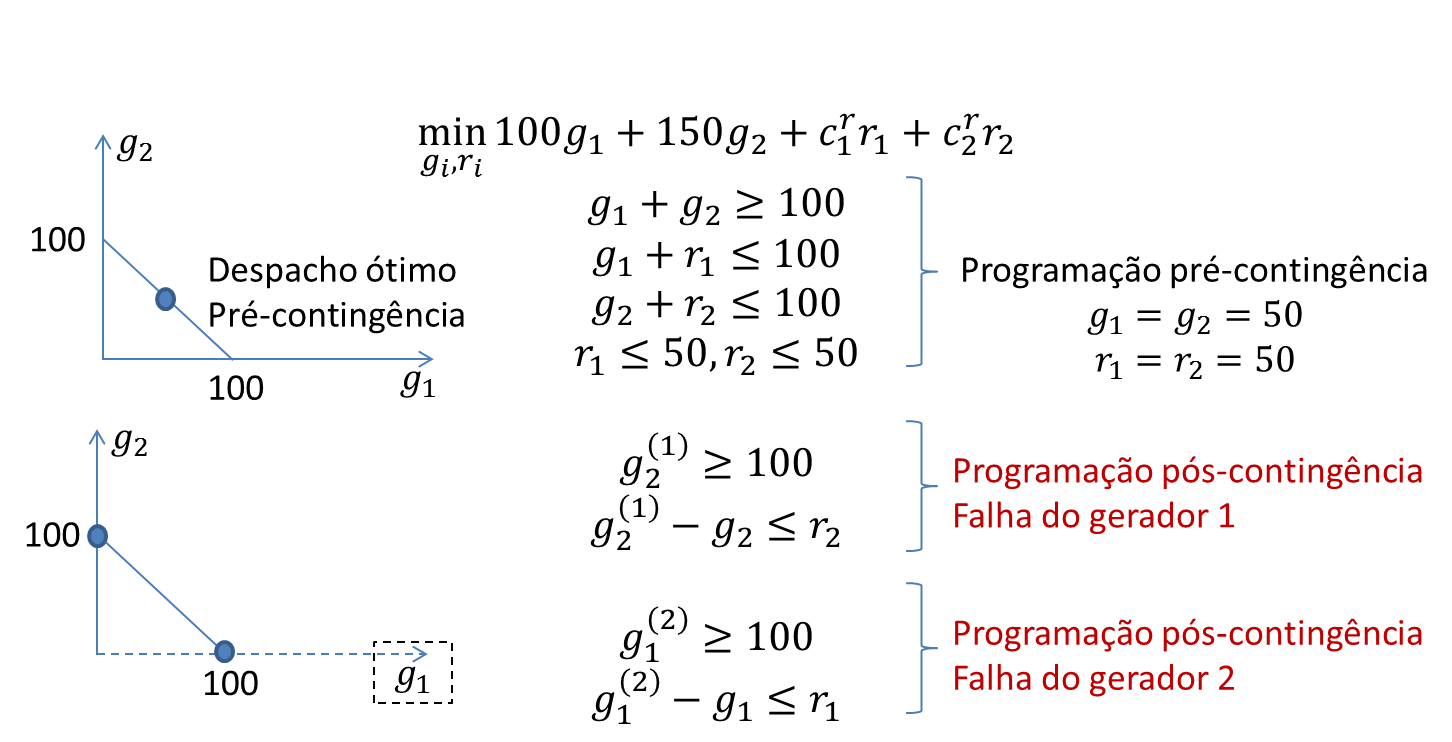
\includegraphics[scale=0.5]{aula4-27}\protect\caption{\label{fig:aula4-27} Falhar qualquer estado pós-contingência }
\end{centering}
\end{figure}

O despacho de potência e reservas apresentado de maneira geral pode ser expresso de algumas formas
%%\begin{itemize}
O critério de confiabilidade $n-k$ significa que fazemos a programação pré-contingência de modo que garantimos o pleno atendimento da demanda prevista mesmo que até $k$ componentes do sistema falhem. 
Esse critério, no entanto, deve levar em consideração quando há componentes que dependem de outros para estarem em funcionamento. Por exemplo, se há um gerador numa barra cujos transmissores falhem, então essa gerador também terá falhado do ponto de vista do sistema.

O critério $n-k$ pode ser modelado através da restrição a seguir: 
$$\sum_{i\in U}a_{i}^{G}(k)+\sum_{l\in L}a_{l}^{L}(k)\geq n-K$$
em que pelo $a(k)$ é vetor de disponibilidade: vale 1 se o elemento está disponível e zero caso contrário (sendo os sobrescrito $G$ e $L$ referentes aos geradores e linhas de transmissão, respectivamente):
$$a(k)=\left[a^{G}(k)|a^{L}(k)\right]\in\{0,1\}^{n}.$$

%\end{itemize}
Unindo todos os elementos apresentados anteriormente, introduzimos a modelagem completa na figura \ref{fig:aula4-29}.
\begin{figure}[H]
\begin{centering}
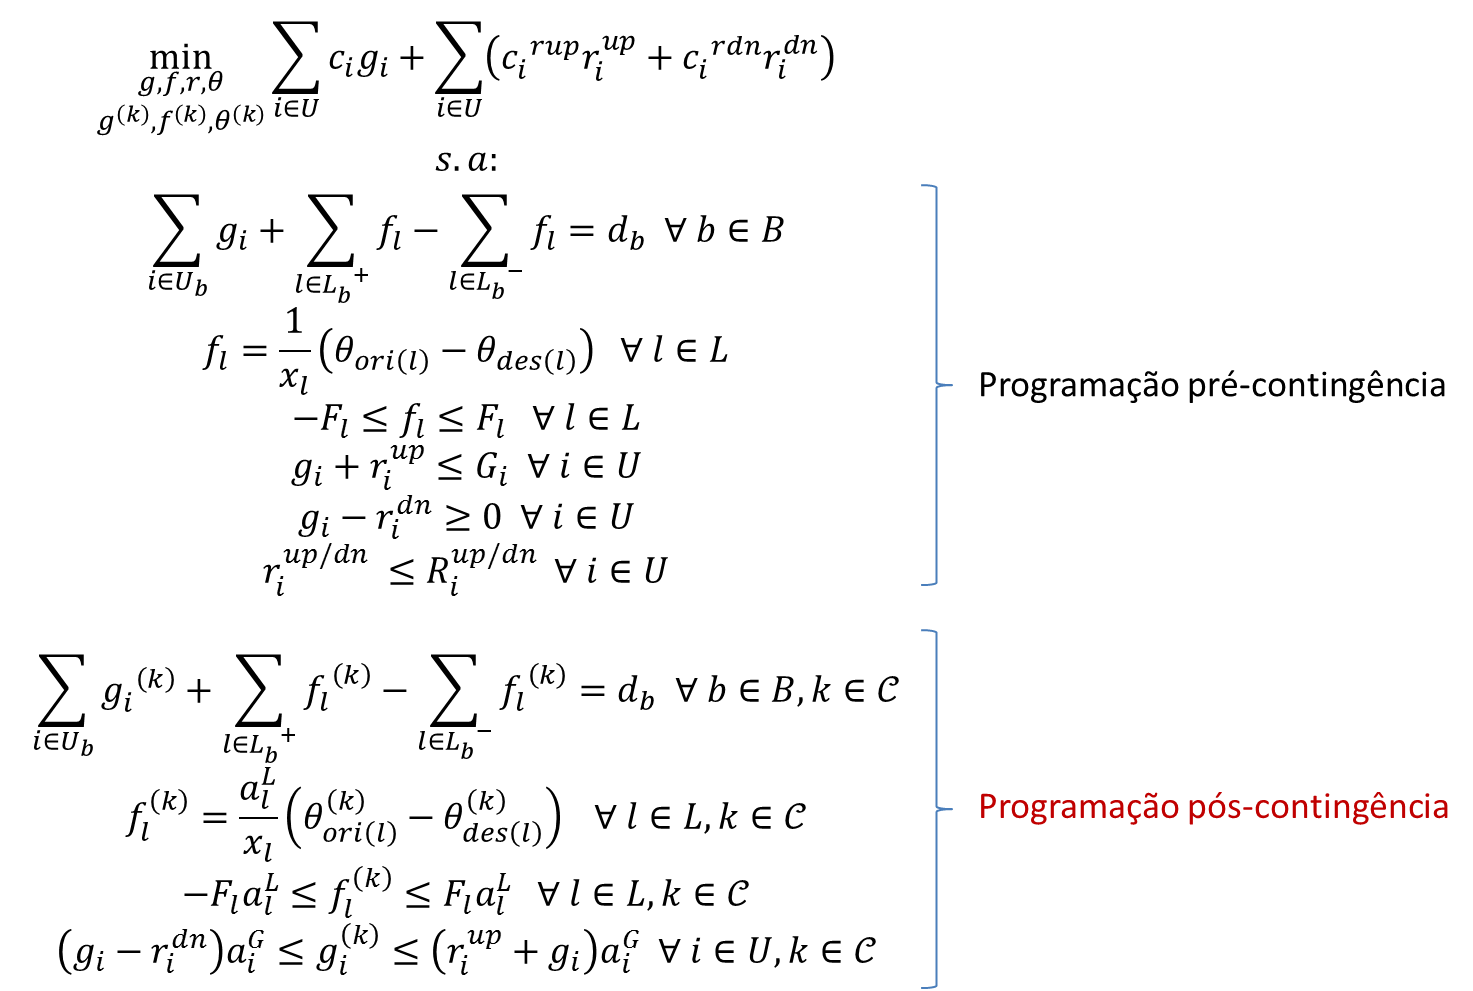
\includegraphics[scale=0.5]{aula4-28}\protect\caption{\label{fig:aula4-28} Problema completo}
\end{centering}
\end{figure}
Considerando todo cenário de demanda líquida:
\begin{figure}[H]
\begin{centering}
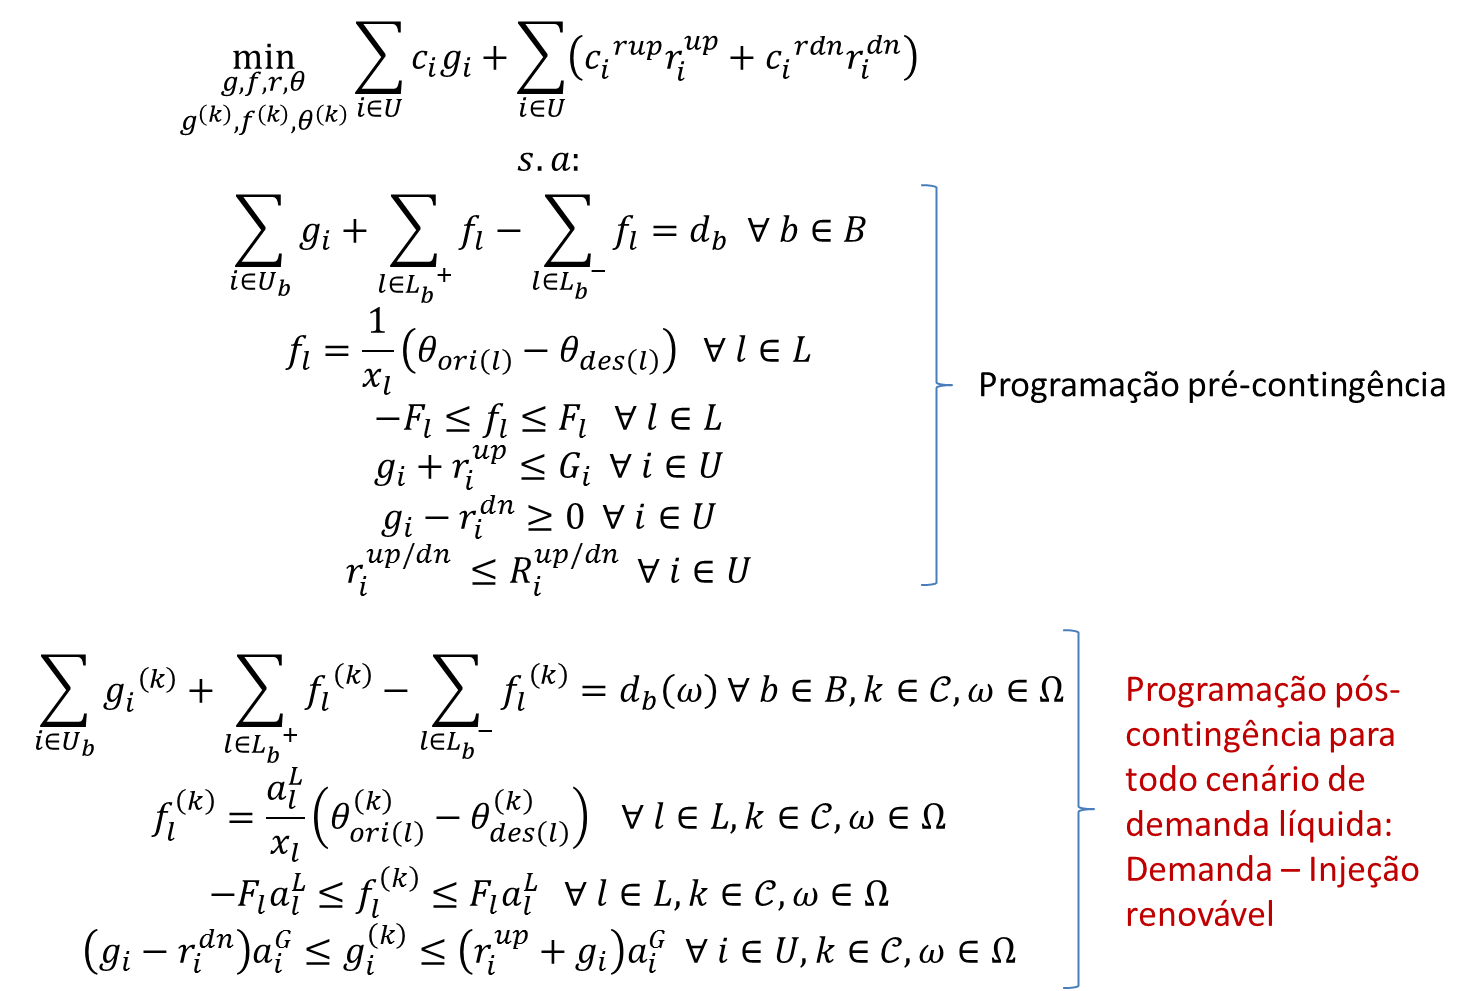
\includegraphics[scale=0.5]{aula4-29}\protect\caption{\label{fig:aula4-29} Problema completo considerando todo cenário de demanda líquida}
\end{centering}
\end{figure}


%Garantir a confiabilidade do sistema energético, é claro, possui um custo. 
O preço da energia está associado ao incremento de custo devido a
um incremento na demada dado por:
\[
\pi_{b}=\pi_{b}^{pre}+\sum_{k\in C}\pi_{bk}^{pos}\forall b\in B,
\]
onde $\pi_{b}^{pre}$ e $\pi_{bk}^{pos}$ são as variáveis duais das
restrições a seguir:
\[
\sum_{i\in U_{b}}g_{i}+\sum_{l\in L_{b}^{+}}f_{l}-\sum_{l\in L_{b}^{-}}f_{l}=d_{b}(\pi_{b}^{pre})\forall b\in B
\]
\[
\sum_{i\in U_{b}}g_{i}^{(k)}+\sum_{l\in L_{b}^{+}}f_{l}^{(k)}-\sum_{l\in L_{b}^{-}}f_{l}^{(k)}=d_{b}(\pi_{b}^{pos})\forall b\in B,k\in C
\]

%\end{itemize}

\subsection{Unit Commitment}

Quando um gerador possui um perfil de produção intermitente, ele incorre em custos de ligar e desligar. Este custo é chamado de \textbf{custo de rampa}, e incide tanto para ligar uma usina como para desligar. Assim, o ato de ligar (desligar) a usina $i$ no tempo $t$ é expresso por $x_{it}^{on}$ ($x_{it}^{off}$). Estando ligado, temos que $v_{it} = 1$, e $0$ caso contrário.

Para fazer sentido temporalmente, devemos introduzir restrições que liguem essas variáveis:
\[
v_{it}-v_{it-1}=x_{it}^{on}-x_{it}^{off}=1-0
\]
\[
-\Delta_{i}^{dn}\leq g_{it+1}-g_{it}\leq\Delta_{i}^{up}
\]
\begin{figure}[H]
\begin{centering}
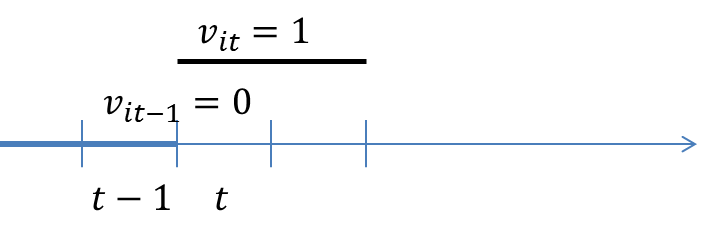
\includegraphics[scale=0.5]{aula4-30}\protect\caption{\label{fig:aula4-30} }
\end{centering}
\end{figure}
 \[
v_{it}-v_{it-1}=x_{it}^{on}-x_{it}^{off}=0-1
\]
\begin{figure}[H]
\begin{centering}
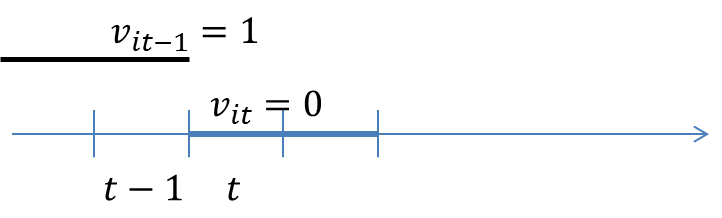
\includegraphics[scale=0.5]{aula4-31}\protect\caption{\label{fig:aula4-31} }
\end{centering}
\end{figure}
%\end{itemize}
\subsection{Operacionalização}

O planejamento da produção da energia elétrica, assim como para diversos outros setores industriais, é feito com diferentes horizontes de tempo.
Quando planeja-se a produção no dia seguinte, utiliza-se modelos de \textit{unit commitment} (figura \ref{fig:aula4-32}). Neste modelo, consideram-se os custo varáveis e fixos de partida, desligamento, restrições de tecnologias, restrições de rede e confiabilidade (segurança). Assim, define-se quais centrais estarão ligadas, em quais horas e suas quantidades de produção nominal e reservas. Nesta etapa, as principais fontes de incerteza são: demanda, geração renovável e disponibilidade de equipamentos.
\begin{figure}[H]
\begin{centering}
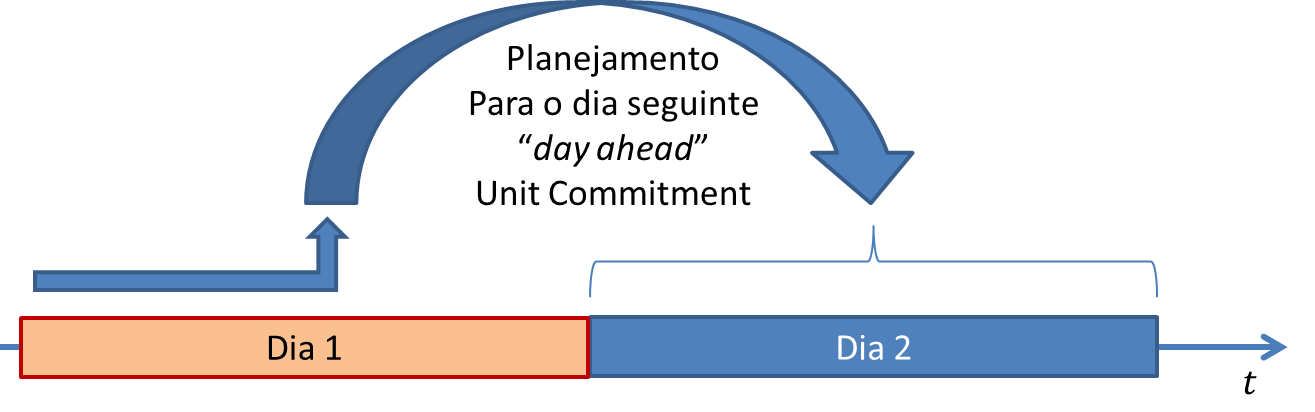
\includegraphics[scale=0.5]{aula4-32}\protect\caption{\label{fig:aula4-32} Planejamento para o dia seguinte }
\end{centering}
\end{figure}

Quando o horizonte de tempo é diminuído para os próximos 5 minutos (figura \ref{fig:aula4-33}), temos a programação da operação em tempo real, em que utiliza-se o modelo de despacho econômico.
Neste modelo, considera-se os custos variáveis, restrições tecnologias,
restrições de rede mais detalhadas e confiabilidade (segurança). Como o horizonte é muito curto, não levamos em conta o custo fixo nem custos de rampa, já que só produzirá quem está ligado no momento exato. Nesta etapa, as principais incertezas são: disponibilidade de equipamentos, injeção intermitente (renováveis).
%\end{itemize}
\begin{figure}[H]
\begin{centering}
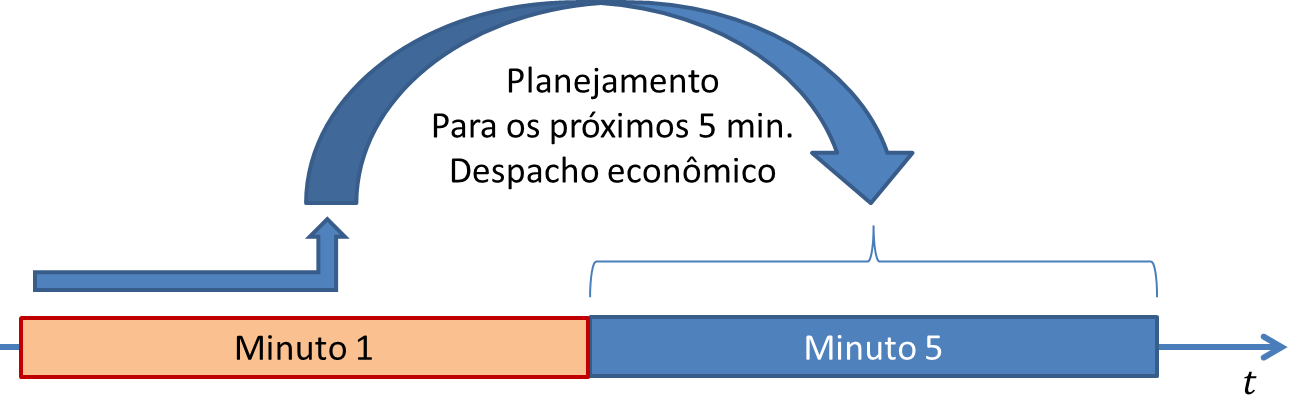
\includegraphics[scale=0.5]{aula4-33}\protect\caption{\label{fig:aula4-33} Operação em tempo real}
\end{centering}
\end{figure}